\documentclass[14pt]{extbook}
\usepackage{multicol, enumerate, enumitem, hyperref, color, soul, setspace, parskip, fancyhdr} %General Packages
\usepackage{amssymb, amsthm, amsmath, bbm, latexsym, units, mathtools} %Math Packages
\everymath{\displaystyle} %All math in Display Style
% Packages with additional options
\usepackage[headsep=0.5cm,headheight=12pt, left=1 in,right= 1 in,top= 1 in,bottom= 1 in]{geometry}
\usepackage[usenames,dvipsnames]{xcolor}
\usepackage{dashrule}  % Package to use the command below to create lines between items
\newcommand{\litem}[1]{\item#1\hspace*{-1cm}\rule{\textwidth}{0.4pt}}
\pagestyle{fancy}
\lhead{Progress Quiz 4}
\chead{}
\rhead{Version B}
\lfoot{4378-7085}
\cfoot{}
\rfoot{Fall 2020}
\begin{document}

\begin{enumerate}
\litem{
Describe the end behavior of the polynomial below.\[ f(x) = -7(x + 8)^{3}(x - 8)^{6}(x + 2)^{3}(x - 2)^{3} \]\begin{enumerate}[label=\Alph*.]
\begin{multicols}{2}\item 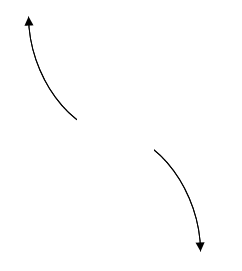
\includegraphics[width = 0.3\textwidth]{../Figures/polyEndBehaviorCopyAB.png}\item 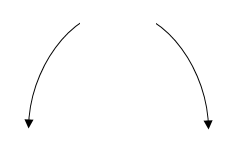
\includegraphics[width = 0.3\textwidth]{../Figures/polyEndBehaviorCopyBB.png}\item 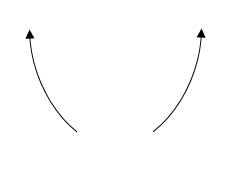
\includegraphics[width = 0.3\textwidth]{../Figures/polyEndBehaviorCopyCB.png}\item 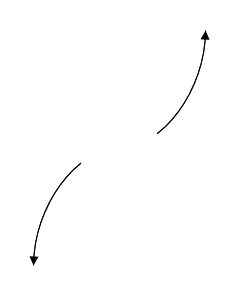
\includegraphics[width = 0.3\textwidth]{../Figures/polyEndBehaviorCopyDB.png}\end{multicols}\item None of the above.
\end{enumerate} }
\litem{
Construct the lowest-degree polynomial given the zeros below. Then, choose the intervals that contain the coefficients of the polynomial in the form $ax^3+bx^2+cx+d$.\[ \frac{-4}{5}, \frac{-1}{5}, \text{ and } \frac{-4}{3} \]\begin{enumerate}[label=\Alph*.]
\item \( a \in [74, 76], b \in [53, 57], c \in [-76, -63], \text{ and } d \in [-16, -13] \)
\item \( a \in [74, 76], b \in [175, 179], c \in [112, 115], \text{ and } d \in [16, 17] \)
\item \( a \in [74, 76], b \in [175, 179], c \in [112, 115], \text{ and } d \in [-16, -13] \)
\item \( a \in [74, 76], b \in [-175, -173], c \in [112, 115], \text{ and } d \in [-16, -13] \)
\item \( a \in [74, 76], b \in [22, 27], c \in [-91, -82], \text{ and } d \in [16, 17] \)

\end{enumerate} }
\litem{
Describe the zero behavior of the zero $x = 5$ of the polynomial below.\[ f(x) = 2(x + 5)^{9}(x - 5)^{14}(x + 4)^{3}(x - 4)^{4} \]\begin{enumerate}[label=\Alph*.]
\begin{multicols}{2}\item 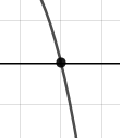
\includegraphics[width = 0.3\textwidth]{../Figures/polyZeroBehaviorAB.png}\item 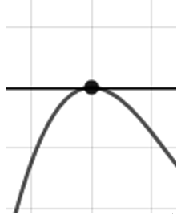
\includegraphics[width = 0.3\textwidth]{../Figures/polyZeroBehaviorBB.png}\item 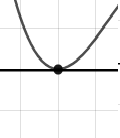
\includegraphics[width = 0.3\textwidth]{../Figures/polyZeroBehaviorCB.png}\item 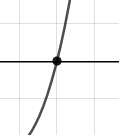
\includegraphics[width = 0.3\textwidth]{../Figures/polyZeroBehaviorDB.png}\end{multicols}\item None of the above.
\end{enumerate} }
\litem{
Describe the end behavior of the polynomial below.\[ f(x) = 7(x + 8)^{5}(x - 8)^{8}(x - 5)^{4}(x + 5)^{4} \]\begin{enumerate}[label=\Alph*.]
\begin{multicols}{2}\item 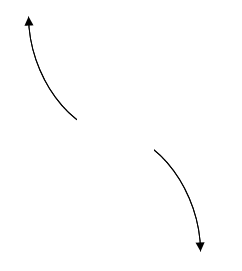
\includegraphics[width = 0.3\textwidth]{../Figures/polyEndBehaviorAB.png}\item 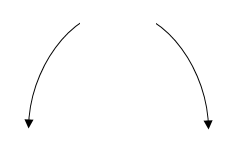
\includegraphics[width = 0.3\textwidth]{../Figures/polyEndBehaviorBB.png}\item 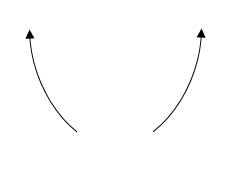
\includegraphics[width = 0.3\textwidth]{../Figures/polyEndBehaviorCB.png}\item 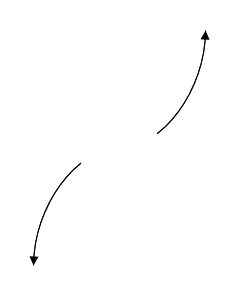
\includegraphics[width = 0.3\textwidth]{../Figures/polyEndBehaviorDB.png}\end{multicols}\item None of the above.
\end{enumerate} }
\litem{
Construct the lowest-degree polynomial given the zeros below. Then, choose the intervals that contain the coefficients of the polynomial in the form $x^3+bx^2+cx+d$.\[ 3 + 4 i \text{ and } -3 \]\begin{enumerate}[label=\Alph*.]
\item \( b \in [-6.9, -0.4], c \in [5.58, 7.49], \text{ and } d \in [71.2, 77.6] \)
\item \( b \in [-0.2, 1.3], c \in [-0.66, 2.32], \text{ and } d \in [-10.7, -7.6] \)
\item \( b \in [1.9, 4.8], c \in [5.58, 7.49], \text{ and } d \in [-77.3, -73.5] \)
\item \( b \in [-0.2, 1.3], c \in [-2.47, -0.78], \text{ and } d \in [-13.7, -9.8] \)
\item \( \text{None of the above.} \)

\end{enumerate} }
\litem{
Construct the lowest-degree polynomial given the zeros below. Then, choose the intervals that contain the coefficients of the polynomial in the form $ax^3+bx^2+cx+d$.\[ -7, \frac{1}{3}, \text{ and } \frac{5}{2} \]\begin{enumerate}[label=\Alph*.]
\item \( a \in [4, 11], b \in [-55, -52], c \in [80, 87], \text{ and } d \in [29, 36] \)
\item \( a \in [4, 11], b \in [-66, -57], c \in [118, 125], \text{ and } d \in [-41, -31] \)
\item \( a \in [4, 11], b \in [-25, -20], c \in [-122, -107], \text{ and } d \in [-41, -31] \)
\item \( a \in [4, 11], b \in [19, 27], c \in [-122, -107], \text{ and } d \in [29, 36] \)
\item \( a \in [4, 11], b \in [19, 27], c \in [-122, -107], \text{ and } d \in [-41, -31] \)

\end{enumerate} }
\litem{
Which of the following equations \textit{could} be of the graph presented below?
\begin{center}
    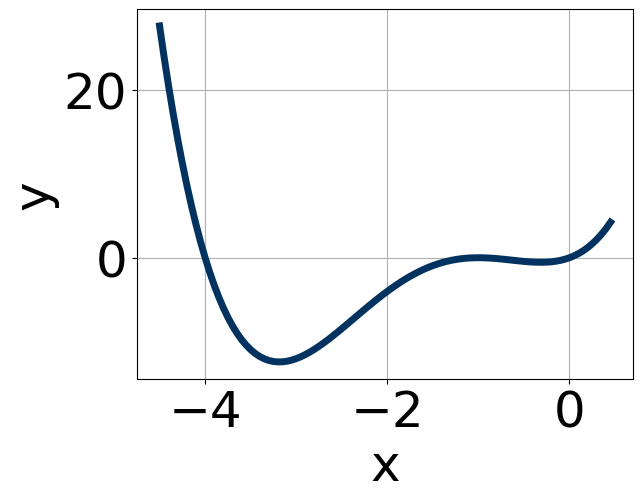
\includegraphics[width=0.5\textwidth]{../Figures/polyGraphToFunctionCopyB.png}
\end{center}
\begin{enumerate}[label=\Alph*.]
\item \( 7x^{9} (x + 1)^{7} (x + 2)^{5} \)
\item \( -7x^{9} (x + 1)^{10} (x + 2)^{11} \)
\item \( 3x^{11} (x + 1)^{8} (x + 2)^{7} \)
\item \( -20x^{7} (x + 1)^{5} (x + 2)^{9} \)
\item \( -3x^{5} (x + 1)^{10} (x + 2)^{8} \)

\end{enumerate} }
\litem{
Describe the zero behavior of the zero $x = 3$ of the polynomial below.\[ f(x) = 8(x - 6)^{11}(x + 6)^{8}(x + 3)^{7}(x - 3)^{2} \]\begin{enumerate}[label=\Alph*.]
\begin{multicols}{2}\item 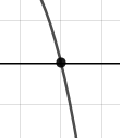
\includegraphics[width = 0.3\textwidth]{../Figures/polyZeroBehaviorCopyAB.png}\item 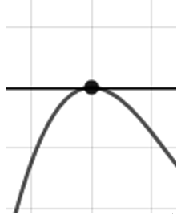
\includegraphics[width = 0.3\textwidth]{../Figures/polyZeroBehaviorCopyBB.png}\item 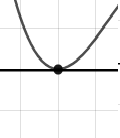
\includegraphics[width = 0.3\textwidth]{../Figures/polyZeroBehaviorCopyCB.png}\item 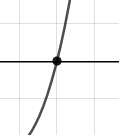
\includegraphics[width = 0.3\textwidth]{../Figures/polyZeroBehaviorCopyDB.png}\end{multicols}\item None of the above.
\end{enumerate} }
\litem{
Construct the lowest-degree polynomial given the zeros below. Then, choose the intervals that contain the coefficients of the polynomial in the form $x^3+bx^2+cx+d$.\[ -4 + 4 i \text{ and } 4 \]\begin{enumerate}[label=\Alph*.]
\item \( b \in [-2.3, 2.2], c \in [-3, 10], \text{ and } d \in [-22, -15] \)
\item \( b \in [-2.3, 2.2], c \in [-14, -6], \text{ and } d \in [11, 19] \)
\item \( b \in [-5.4, -1], c \in [-3, 10], \text{ and } d \in [123, 134] \)
\item \( b \in [2.1, 5.3], c \in [-3, 10], \text{ and } d \in [-138, -126] \)
\item \( \text{None of the above.} \)

\end{enumerate} }
\litem{
Which of the following equations \textit{could} be of the graph presented below?
\begin{center}
    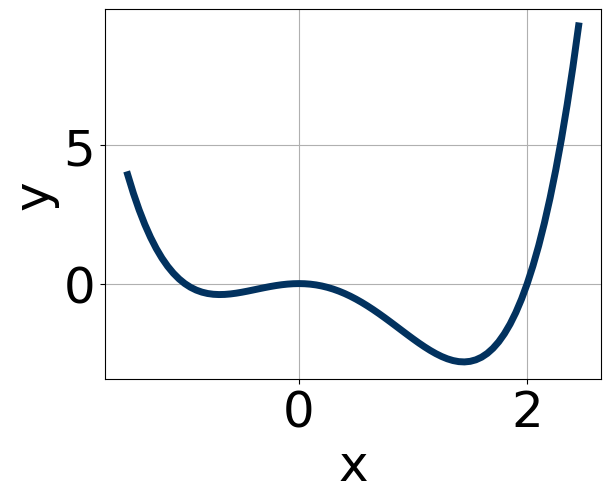
\includegraphics[width=0.5\textwidth]{../Figures/polyGraphToFunctionB.png}
\end{center}
\begin{enumerate}[label=\Alph*.]
\item \( 9x^{8} (x + 3)^{6} (x - 2)^{11} \)
\item \( 10x^{9} (x + 3)^{6} (x - 2)^{11} \)
\item \( -14x^{11} (x + 3)^{10} (x - 2)^{7} \)
\item \( -10x^{9} (x + 3)^{5} (x - 2)^{7} \)
\item \( 3x^{5} (x + 3)^{9} (x - 2)^{5} \)

\end{enumerate} }
\end{enumerate}

\end{document}